\subsection{Descrizione delle classi}
Vengono descritte di seguito le classi principali, iniziando da quelle che costituiscono il modello dati. Successivamente vengono descritte le classi utility che permettono la gestione di elementi comuni alle varie parti dell'app, infine le Activity che compongono l'applicazione.

\subsubsection{Classi del modello dati}
Il modello dati del gioco è rappresentato in figura \ref{fig:class}.

\begin{figure}[h!]
\centering{
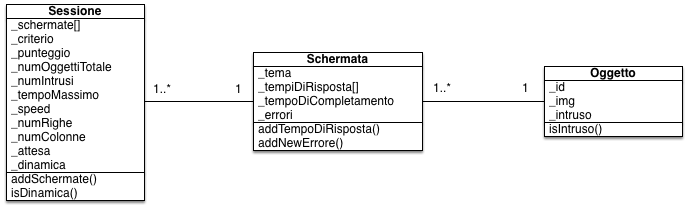
\includegraphics[width=\textwidth]{class.png}}
\caption{Class Diagram del modello dati}
\label{fig:class}
\end{figure}

\begin{itemize}
\item \textbf{Oggetto} è la classe che rappresenta il singolo oggetto sullo stage di gioco.
\item \textbf{Schermata} è la classe che rappresenta la singola schermata di gioco. Una schermata contiene da 1 a N oggetti (N è definito in base alla modalità di gioco)
\item \textbf{Sessione} è la classe che rappresenta l'intera sessione di gioco. Una sessione è costituita da una o più schermate.
\end{itemize}

Tutte le classi sopracitate, oltre ai metodi particolari riportati nello schema, espongono anche i relativi metodi getter e setter per accedere agli attributi.
\subsubsection{Classi utility}

\begin{itemize}
\item \code{DbAdapter} e \code{DatabaseHelper} sono due classi che contengono i metodi per la gestione del database delle email (le email da inviare al termine della partita vengono salvate in una tabella che agisce da coda di invio, per ogni email viene salvato il testo e l'indirizzo email di destinazione).
\item \code{GmailSender} è la classe che contiene la logica per poter inviare il report della sessione di gioco via mail. Questa classe utilizza la classe \code{JSSEProvider} per gestire l'autenticazione nella connessione al server di posta in uscita.
\item \code{ImgUtils} contiene alcuni metodi per la gestione delle immagini all'interno del gioco
\item \code{JsonUtils} contiene i metodi per accedere alle strutture dati JSON che definiscono le possibili schermate (v. Strutture Dati)
\item \code{MailUtils} contiene il metodo che spedisce la mail in modalità asincrona, assieme al metodo che compone il messaggio da spedire
\item \code{TimeUtils} contiene il metodo che scrive il tempo in secondi in una stringa nel formato corretto.
\item \code{ViewContainer} e \code{ViewContainerAccessor} sono due classi predefinite per la gestione delle animazioni con la libreria Universal Tween Engine, definiscono il contenitore per la view da animare e il modo in cui dev'essere animata.
\end{itemize}

\subsubsection{Activity}

\begin{itemize}
\item \code{MainActivity} è l'activity presentata all'avvio dell'app, propone le due modalità di gioco e il setup.
\item \code{SetupActivity} è l'activity che consente di modificare i parametri di gioco.
\item \code{ModeOneActivity} è l'activity che esegue la modalità di gioco dinamica (con oggetti in movimento)
\item \code{ModeTwoActivity} è l'activity che esegue la modalità di gioco statica (griglia con oggetti fissi nello spazio)
\end{itemize}

La descrizione dei singoli metodi contenuti nelle activity è riportata all'interno del codice.

\subsection{Strutture dati}
All'interno della cartella \code{Assets} sono riportati alcuni file JSON che descrivono le possibili schermate per ogni criterio (forma, percettivo, colore). Ad esempio, il file \code{percettivo.json}:

\begin{lstlisting}[float, caption=Contenuto del file \code{percettivo.json}, label=lst:percettivo_json]
{
    "scene" : [
        {
                 "id" : "universo",
                 "nome" : "Universo",
                 "target" : "stella",
                 "elementi" : [
                        {"nome" : "pianeta_1"},
                        {"nome" : "pianeta_2"},
                        {"nome" : "pianeta_3"}
                 ],
                 "sfondo" : "bg_universo"
        },
        {
                   "id" : "prato",
                   "nome" : "Prato",
                   "target" : "quadrifoglio",
                   "elementi" : [
                          {"nome" : "trifoglio"}
                   ],
                   "sfondo" : "bg_prato"
        },
        {
                 "id" : "natura",
                 "nome" : "Natura",
                 "target" : "tartaruga",
                 "elementi" : [
                        {"nome" : "anguria"}
                 ],
                 "sfondo" : "bg_prato"
        }
    ]
}
\end{lstlisting}

Per ogni scena vengono specificati quali sono gli elementi grafici da utilizzare per comporla.

\subsection{Modello della sessione di gioco}
Nella figura \ref{fig:session} è riportato il flusso di gioco, con riferimento alle attività contenute nelle activity.

\begin{figure}[h!]
\centering{
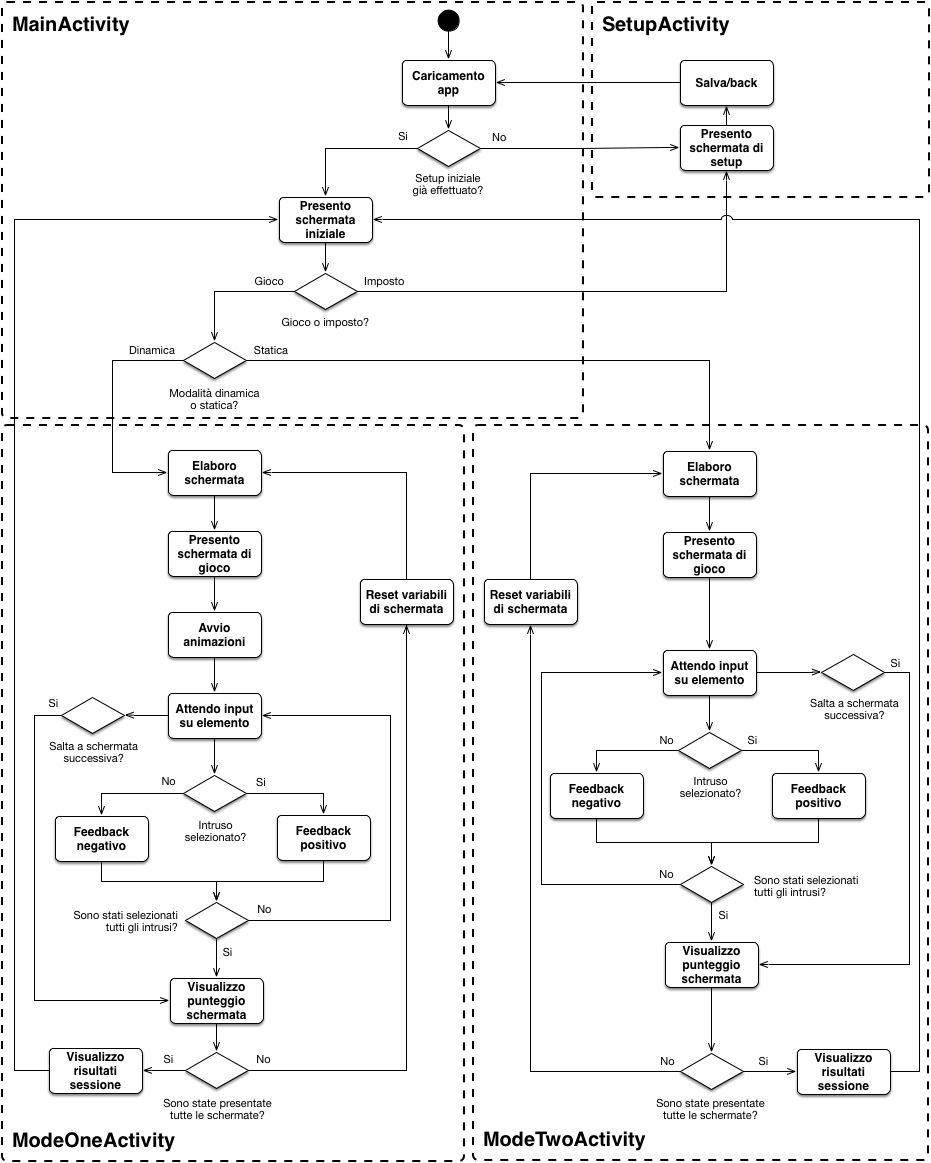
\includegraphics[width=\textwidth]{session.png}}
\caption{Modello della sessione di gioco}
\label{fig:session}
\end{figure}
